\chapter{Lec 10 - Maximum Flows}

\section{Definitions}
A \textbf{flow network} is a directed graph $G = (V, E)$ where each edge has a \textbf{capacity} $c(e) \in \mathbb{R}^+$, along with a designated \textbf{source} $s \in V$ and \textbf{sink} $t \in V$. For convenience, write $c(e) = 0$ if $e \notin E$. We assume that there are no edges entering $s$ and no edges leaving $t$.\newline\newline
A \textbf{flow} is a function $f: E \rightarrow \mathbb{R}^+$ satisfying the following constraints:
\begin{itemize}
    \item capacity: $\forall e \in E \,\, f(e) \leq c(e)$
    \item conservation: $\forall u \in V \setminus \{s, t\}$ we have $\sum_{v \in V \, s.t.\, (v, u) \in E}f(v, u) = \sum_{v \in V \, s.t.\, (u, v) \in E}f(u, v)$. Basically, the flow that \textit{enters} in a node must be equal to the flow that \textit{goes out} from that node.
\end{itemize}
The \textbf{value} of a flow is $|f| = \sum_{v \in V \, s.t. \, (s,v) \in E}f(s,v)$ that is, the total flow out of the source.

\section{Maximum flow problem}
Given a flow network, find a flow of \textbf{maximum value}.\newline\newline
\textbf{Applications:}
\begin{itemize}
    \item Rail networks
    \item Road networks
    \item Electrical networks
    \item ...
\end{itemize}
Max flow reduces to linear programming (like many other problems), but there are more efficient algorithms. We'll see one of them (Ford-Fulkerson), but there are plenty of more efficient algorithms. \newline\newline
A first simple algorithm can be the following:
\begin{enumerate}
    \item Find a path from $s$ to $t$ (in linear time using BFS)
    \item Find the \textit{bottleneck} edge (i.e. the edge with smallest capacity in the path) and send as much flow along the path as possible.
    \item Update capacities
    \item Remove edges that have 0 remaining capacity
    \item Repeat until the graph has no more $s-t$ paths
\end{enumerate}
Actually, this algorithm will \textbf{not} always work. We can improve it by exploiting the following idea: revise/undo some of the flow later in the algorithm by \textit{pushing back} some flow through new edges in the reverse direction.

\section{Ford-Fulkerson method}
\textbf{Definition:}\newline
Given a flow network $G$ and a flow $f$, the \textbf{residual network} of $G$ with respect to $f$, $G_f$, is a network with vertex set $V$ and edge set $E_r$ as follows:\newline
For every edge $e = (u, v)$ in $G$:
\begin{enumerate}
    \item if $f(e) < c(e)$, add $e$ to $G_f$ with capacity $c_f(e) = c(e) - f(e)$

    \item if $f(e) > 0$, add another edge $(v, u)$ to $G_f$ with capacity $c_f(e) = f(e)$
\end{enumerate}
Intuitively, the residual network $G_f$ consists of edges with capacities that represent how we can change the flow on edges of $G$.\newline\newline
The residual network $G_f$ may also contain edges that are not in $G$. As an algorithm manipulates the flow, with the goal of increasing the total flow, it might need to decrease the flow on a particular edge. In order to represent a possible decrease of a positive flow $f(u, v)$ on an edge in $G$, we place an edge $v, u$ into $G_f$ with residual capacity $c_f(v, u) = f(u, v)$. Sending flow back along an edge is equivalent to \textit{decreasing} the flow on the edge.\newline\newline
The Ford-Fulkerson method repeatedly finds an $s-t$ path $P$ in $G_f$ (e.g. using BFS) and uses $P$ to \textbf{increase} the current flow. $P$ is called \textbf{augmenting path}.

\begin{algorithm}
\caption{Ford-Fulkerson}\label{Ford-Fulkerson}
    \begin{algorithmic}[1]
    \Procedure{Ford-Fulkerson($G, s, t$)}{}
        \State initialize the $f(e) = 0\,\, \forall e \in G.E$
        \State $G_f = G$
        \While{There exists an augmenting path $P$ in $G_f$}
            \State $\Delta p = min_{e \in P}(c_f(e)) \quad //\Delta p \text{ is the bottleneck capacity in }P$

            \For{\textbf{each} edge $e = (u, v) \in P$}
                \If{$(u, v) \in G.E$}
                    \State $f(u, v) = f(u, v) + \Delta p$
                \Else
                    \State $f(v, u) = f(v, u) - \Delta p \quad // \text{if the edge $(u, v) \notin G.E$, the opposite edge $(v, u)$ must be in $E$}$
                \EndIf
            \EndFor
            \State Update the residual graph $G_f$
        \EndWhile
    \EndProcedure   
    \end{algorithmic}
\end{algorithm}
\begin{center}
    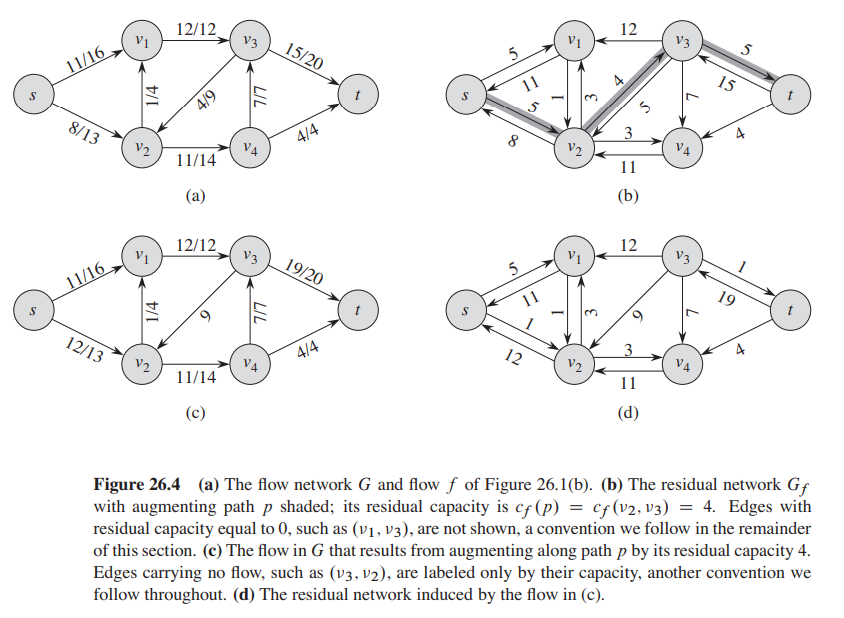
\includegraphics[scale = 0.8]{images/Ford-Fulk.png}
\end{center}
Basically, when we find an augmenting path $P$:
\begin{itemize}
    \item if an edge $(u, v) \in E$, we are increasing its flow by the bottleneck capacity

    \item if an edge $(u, v) \notin E$, it's like we are decreasing the flow on the edge $(v, u)$ and adding that \textit{amount} of flow to other edges 
\end{itemize}
\textbf{Complexity:}
\begin{itemize}
    \item The flow value increases by $\geq 1$ at each iteration.

    \item The complexity of each iteration is $O(m)$.
\end{itemize}
The total complexity is $O(m \cdot |f^*|)$ where $|f^*|$ is a max flow.
